\documentclass[11pt,a4paper]{article}
\usepackage[margin=25mm]{geometry}
\usepackage[T1]{fontenc}
\usepackage[utf8]{inputenc}
\usepackage{lmodern}
\usepackage{microtype}
\usepackage{amsmath,amssymb}
\usepackage{booktabs,array,tabularx}
\usepackage{graphicx}
\usepackage{float}
\usepackage{caption}
\usepackage{hyperref}
\usepackage{fancyhdr}
\usepackage{setspace}
\hypersetup{colorlinks=true,linkcolor=blue,urlcolor=blue,citecolor=blue}
\graphicspath{{../results/figures/}}
\setstretch{1.12}
\setlength{\parskip}{5pt}
\setlength{\parindent}{0pt}
\pagestyle{fancy}
\fancyhf{}
\lhead{Indian district night-light growth}
\rhead{Research report}
\cfoot{\thepage}
\renewcommand{\headrulewidth}{0.3pt}

\title{Spatial Patterns in Indian District Night-Light Growth\\
\large Descriptive Statistics, Spatial Econometrics, and Cluster Analysis}
\author{Nakshatra Ghosh}
\date{1 October 2026}

\begin{document}
\maketitle
\begin{abstract}
This study examines annual night-light growth across 640 Indian Census 2011 districts using the SHRUG v2.2 data platform. The principal comparison uses consistently processed VIIRS observations from 2013 to 2021 and fixed 2011 population as a size normalizer. Districts with lower initial normalized light tend to have faster subsequent light growth: the conditional ordinary least squares (OLS) coefficient is $-0.0457$ per year (HC3 standard error 0.00344). Growth is strongly spatially clustered (global Moran's $I=0.654$, 999-permutation $p=0.001$). Spatial lag, spatial error, and spatial Durbin models distinguish several forms of dependence. The Durbin model reduces residual Moran's $I$ to $-0.0037$ ($p=0.935$), although its estimated indirect impact of initial light is imprecise. A local Moran map and a spatially constrained three-region typology describe where growth clusters occur. These results concern satellite light, not measured district GDP, and do not identify causal spillovers.
\end{abstract}

\tableofcontents
\clearpage

\section{Research question and interpretation}
The first project in the supplied brief asks whether Indian districts with lower initial development grew faster, whether growth is geographically clustered, and whether the trajectory of one district is related to its neighbors. We answer these questions using district total night-light intensity as an imperfect proxy for local economic activity. Night lights can reflect electrification, settlement patterns, infrastructure, and measurement changes as well as economic output \cite{henderson2012,asher2021}. No district GDP is imputed from lights.

The analysis uses 2011 district boundaries throughout, so the unit does not change over time. The main estimand is growth of light per \emph{1,000 baseline (2011) residents}. The denominator is held fixed, because annual district population is not observed. Thus the growth rate equals the growth rate of total district light; the initial normalized level adjusts for baseline district size. It is not annual per-capita income growth.

\section{Data assembly and checks}
The SHRUG v2.2 source files used are the district VIIRS annual light table, the district DMSP calibrated light table, the 2011 district Population Census Abstract, the 2011 district population/area key, and district polygons \cite{shrugviirs,shrugdmsp,shruglicense}. The deposited analysis panels contain 12,800 VIIRS records (640 districts, 10 years, two masking categories) and 12,800 DMSP records (640 districts, 20 years after averaging concurrent satellites). The raw VIIRS file also contains 2022--2023, but the published table documentation describes 2012--2021, which defines our documented analysis range. We do not join the DMSP and VIIRS scales into one series.

The polygon file contains 641 shapes. One is an unlabelled district-000 placeholder absent from all 640 census and light tables; it is excluded. All 640 remaining polygon keys match the census and light panels exactly. We verified unique district-year-category identifiers for VIIRS and district-year-satellite identifiers for DMSP, positive 2011 population and area, complete main covariates, and strictly positive VIIRS light in both main endpoint years. Zeros in 2012 are one reason for choosing 2013 as the log-growth baseline. The first DMSP year with positive calibrated district light for all 640 districts is 2000; the historical check therefore compares 2000 and 2013.

Let $N_i$ denote 2011 census population, $V_{it}$ the SHRUG average-masked VIIRS annual sum, and $D_{it}$ the calibrated DMSP annual sum. We define
\begin{equation}
L_{it}=1000V_{it}/N_i,\qquad z_{it}=\log L_{it},\qquad
g_i=\frac{z_{i,2021}-z_{i,2013}}{8}.
\end{equation}
The denominator is fixed in both endpoints. The 2011 covariates are log population density (population/land area), literacy among those age seven and above, the share of main workers who are cultivators or agricultural laborers, and the population share classified as Scheduled Caste or Scheduled Tribe. These are baseline descriptors, not exogenous instruments. DMSP uses $1000D_{it}/N_i$ only within its own series; calibrated observations from multiple satellites in one year are averaged before analysis.

\section{Numerical and visual descriptives}
\begin{table}[htbp]
\centering\small
\caption{Selected district descriptive statistics ($n=640$)}
\begin{tabular}{lrrrr}
\toprule
Variable & Mean & Median & 10th pct. & 90th pct.\\
\midrule
VIIRS per 1,000 baseline residents, 2013 & 7.689 & 6.068 & 1.641 & 15.259\\
VIIRS per 1,000 baseline residents, 2021 & 11.209 & 9.829 & 4.653 & 18.272\\
Annual log-light growth, 2013--2021 & 0.0682 & 0.0588 & $-0.0004$ & 0.1478\\
2011 population density & 994.0 & 409.8 & 137.7 & 1251.8\\
2011 adult literacy share & 0.723 & 0.722 & 0.590 & 0.854\\
2011 agricultural main-worker share & 0.533 & 0.591 & 0.197 & 0.773\\
\bottomrule
\end{tabular}
\label{tab:desc}
\end{table}

Mean normalized light rises 45.8\% between the endpoint years; its district median rises 62.0\%. Mean annual log growth is 0.0682, while 10.5\% of districts have negative endpoint growth. The distribution is right-skewed, with a maximum annual log rate of 0.380. The annual series shows a visible step between 2016 and 2017, so the long-run average must not be read as a uniform year-by-year gain. Variation in preprocessing or illumination may contribute to that pattern.

\begin{figure}[p]
\centering
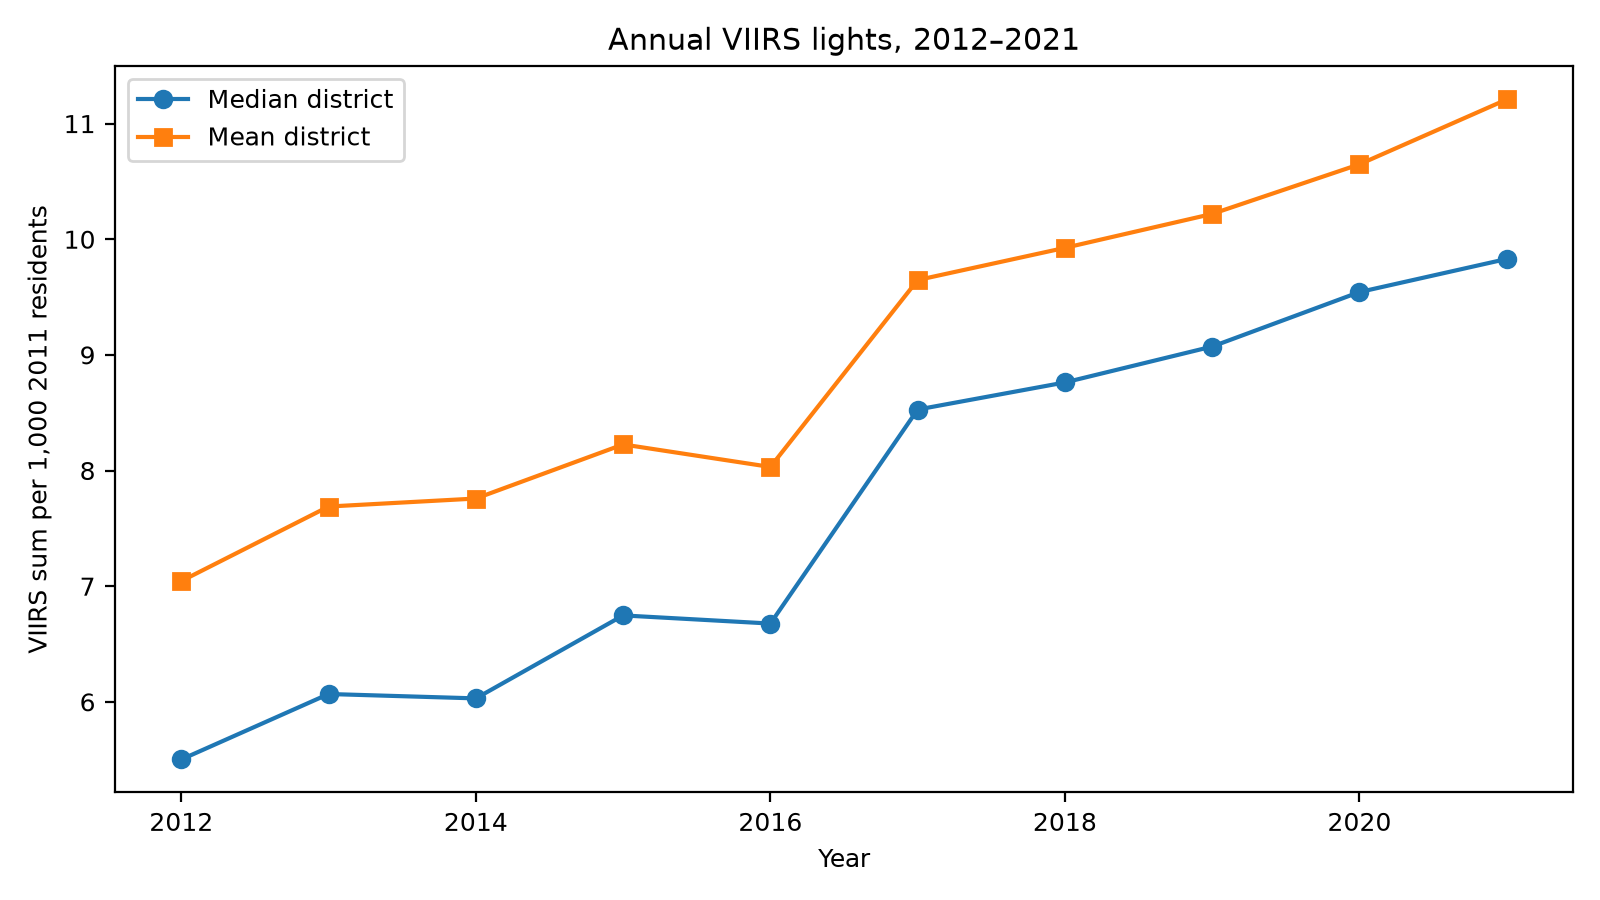
\includegraphics[width=0.84\linewidth]{viirs_trend.png}
\caption{District mean and median VIIRS light normalized by fixed 2011 population.}
\label{fig:trend}
\vspace{7mm}
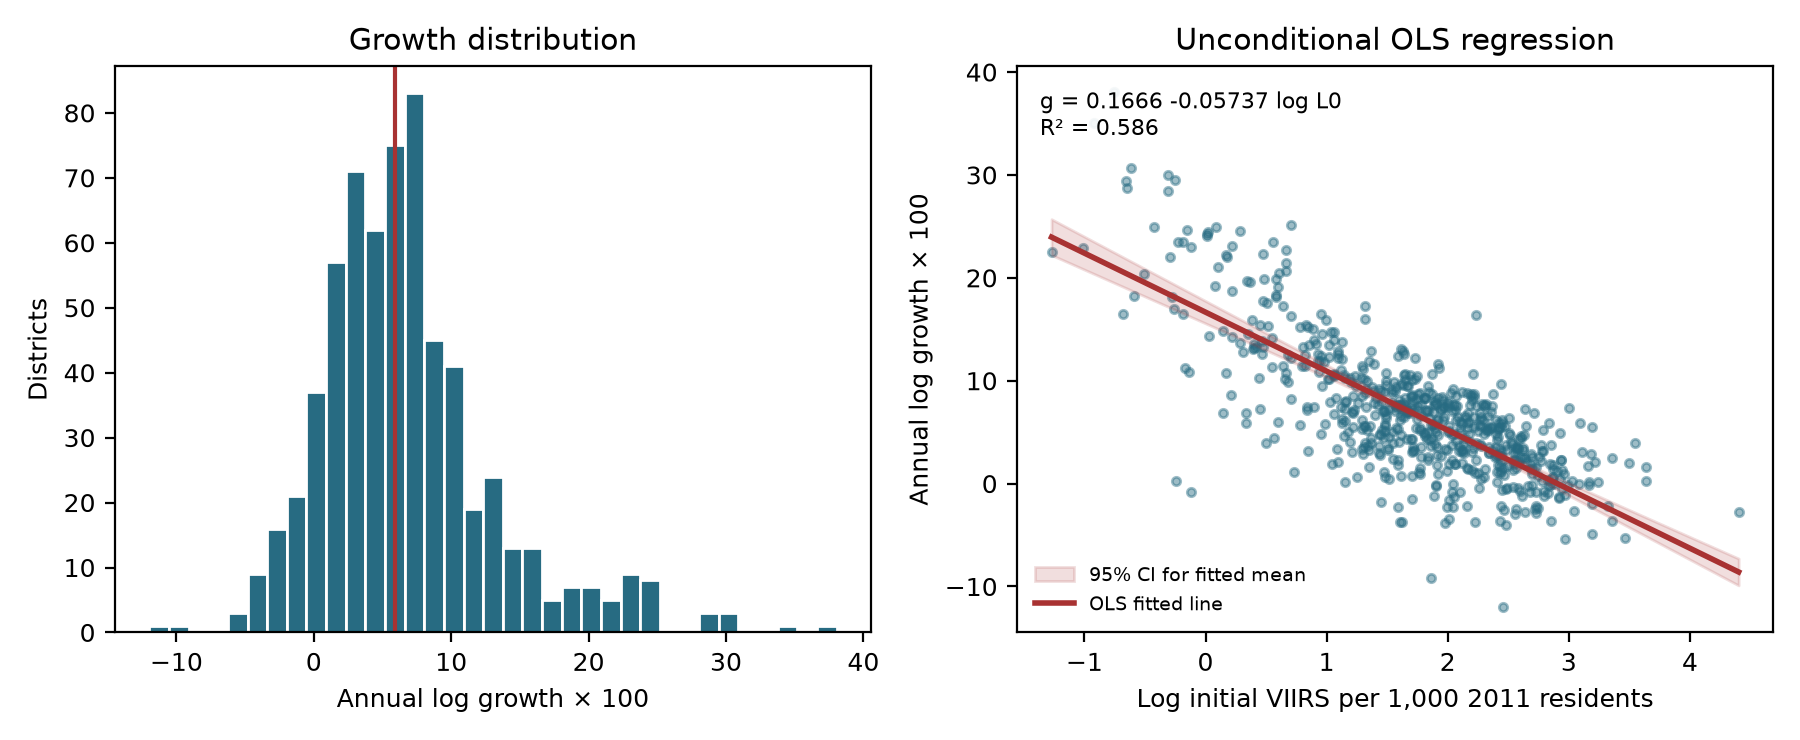
\includegraphics[width=0.95\linewidth]{distribution_convergence.png}
\caption{Distribution of annual endpoint growth and its unconditional OLS regression line. The shaded band is a 95\% confidence interval for the fitted mean, not for individual districts.}
\label{fig:distribution}
\end{figure}

\section{Spatial weights and exploratory clustering}
The primary spatial matrix $W$ assigns equal row-standardized weight to 2011 districts that share at least one polygon boundary point (Queen contiguity). It has 4.14 neighbors per district on average. The supplied geometry yields 34 disconnected components and 12 districts with no contiguous neighbor. For those 12 rows, all weights are zero; we do not fabricate a maritime or other distant boundary. A sensitivity matrix uses eight nearest representative points in equal-area projection EPSG:6933, which is connected but may bridge water or border gaps. The choice of $W$ encodes what ``nearby'' means and is therefore substantively important.

Global Moran's $I$ measures correlation between centered district values and their spatially weighted neighbors. Under spatial randomness its expectation here is approximately $-0.00156$. We use 999 random permutations to obtain two-sided $p$ values. Growth Moran's $I$ is 0.654 ($p=0.001$); initial light Moran's $I$ is 0.612 ($p=0.001$). These reject spatial randomness but cannot distinguish diffusion from geographically clustered common causes.

Local Moran $I_i$ classifies each eligible district as high-high, low-low, high-low, or low-high relative to its contiguous neighbors. We control the false discovery rate over the 628 districts with at least one neighbor using Benjamini--Hochberg at 5\%. There are 37 high-high districts, 37 low-low districts, and two low-high spatial outliers; 552 districts are not significant and 12 have no contiguous neighbor. High-high districts include several in Bihar and Manipur. The cluster labels describe joint local deviations in this period, not enduring administrative regions.

\begin{figure}[p]
\centering
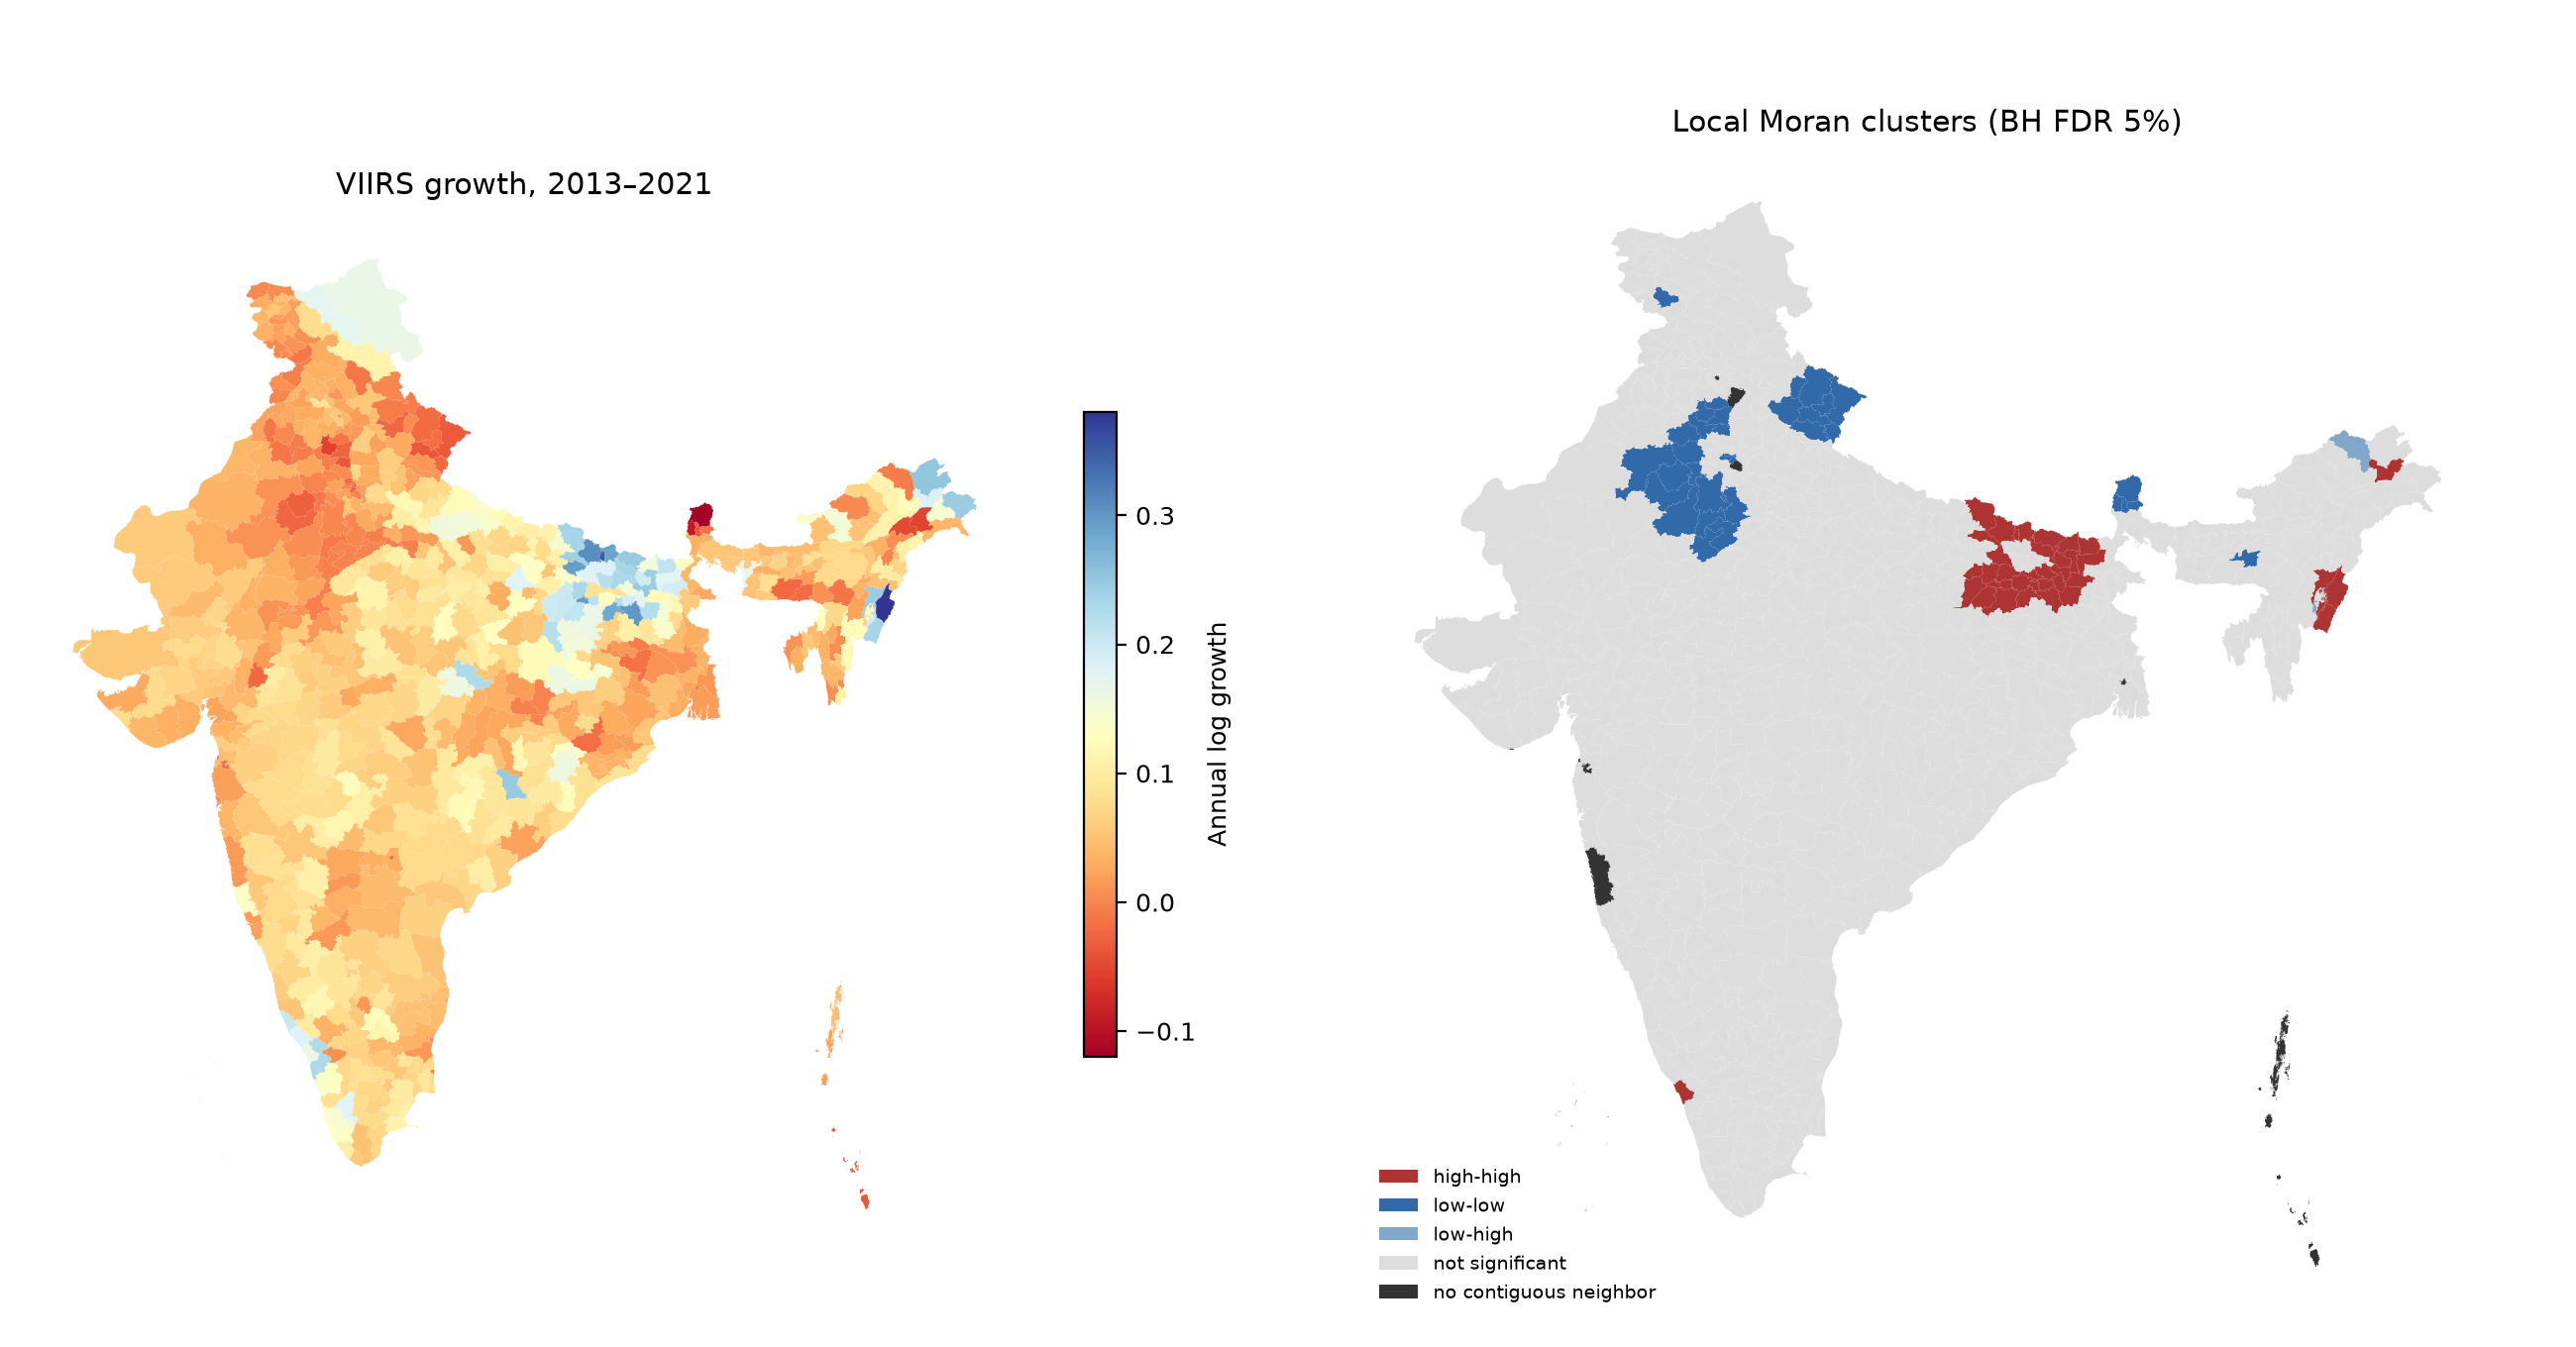
\includegraphics[width=\linewidth]{growth_maps.png}
\caption{Annual 2013--2021 VIIRS log-light growth (left) and local Moran classes after false discovery rate correction (right). Dark gray marks districts with no Queen neighbor.}
\label{fig:maps}
\end{figure}

To complement local significance tests, we standardize initial log light, annual growth, log density, literacy, and agricultural employment share and perform Ward agglomerative clustering. Merges are allowed only along a symmetric eight-nearest-neighbor graph. We compare $k=2,\ldots,6$ using the feature-space silhouette score and select $k=3$ (score 0.158; each selected group is connected in the graph). This low score indicates a useful broad typology rather than sharply separated natural clusters. Growth is itself a clustering input, so differences in group growth are descriptive and provide no independent test.

\begin{table}[htbp]
\centering\small
\caption{Spatially constrained district typology}
\begin{tabular}{lrrrrr}
\toprule
Group & Districts & Mean growth & Mean initial log light & Median density & Mean literacy\\
\midrule
1 & 252 & 0.1023 & 1.443 & 351.6 & 0.659\\
2 & 347 & 0.0406 & 1.999 & 495.5 & 0.768\\
3 & 41 & 0.0924 & 0.997 & 56.6 & 0.736\\
\bottomrule
\end{tabular}
\label{tab:clusters}
\end{table}

\begin{figure}[p]
\centering
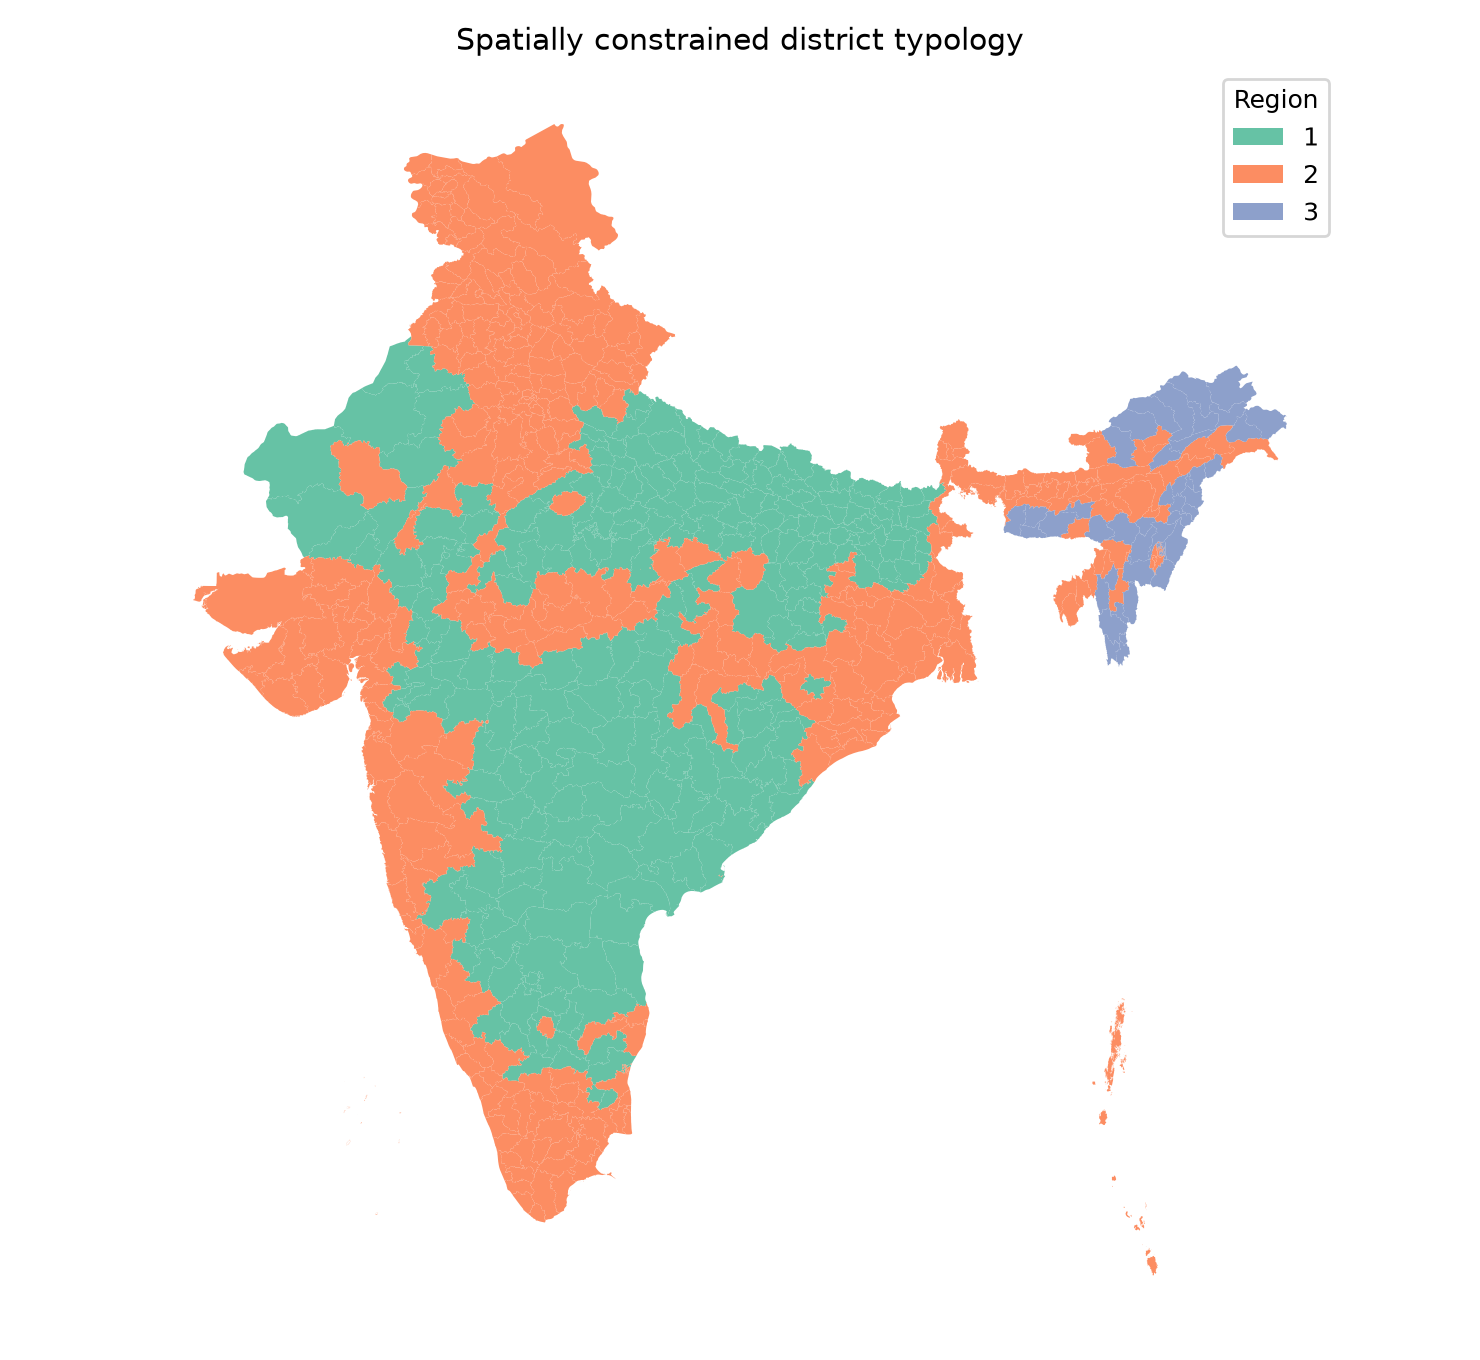
\includegraphics[width=0.75\linewidth]{spatial_regions.png}
\caption{Three spatially constrained Ward groups. The eight-neighbor graph creates contiguous graph regions, which need not be polygon-contiguous everywhere.}
\label{fig:regions}
\end{figure}

\section{Econometric framework}
\subsection{OLS convergence benchmark}
The absolute-convergence regression uses only initial log light, while the conditional specification adds $X_i$ (the four 2011 characteristics) and state indicators $\mu_{s(i)}$:
\begin{equation}
g_i=\alpha+\beta z_{i,2013}+X_i'\gamma+\mu_{s(i)}+\varepsilon_i.
\end{equation}
We report HC3 heteroskedasticity-robust standard errors for OLS. A negative $\beta$ is consistent with lower initially lit districts growing faster conditional on included terms. It does not itself show income convergence. Under the restrictive transitional-growth parameterization $\beta=(e^{-8\lambda}-1)/8$, $\lambda=-\log(1+8\beta)/8$ is an implied annual convergence speed. The transformation is descriptive and inherits all model assumptions.

The red line in Figure~\ref{fig:distribution} is the fitted \emph{unconditional} OLS relation, in annual log-growth units:
\begin{equation}
\widehat g_i=0.16662-0.05737\,z_{i,2013},\qquad R^2=0.586.
\end{equation}
The conditional fitted equation (with state 01 as the omitted indicator) is
\begin{align}
\widehat g_i={}&0.22351-0.04569z_{i,2013}-0.01563\log(\text{density}_{i,2011})\notag\\
&+0.01361\text{literacy}_{i,2011}-0.01720\text{agwork}_{i,2011}
-0.01023\text{SCST}_{i,2011}+\widehat\mu_{s(i)}.
\end{align}
The plot's line and confidence band refer to the simple regression. The conditional equation holds covariates and the state indicator fixed; its intercept is a reference-category model term, not a plausible district prediction with all controls set to zero.

\subsection{Spatial lag, error, and Durbin models}
The spatial autoregressive (SAR) model adds simultaneous neighbor growth, $\rho Wg$, to the conditional equation. Maximum likelihood accounts for the simultaneity of $Wg$ with $g$:
\begin{equation}
g=\rho Wg+\alpha\mathbf{1}+\beta z_0+X\gamma+S\mu+\varepsilon.
\end{equation}
The spatial error model (SEM) instead attributes residual spatial dependence to a correlated disturbance, $u=\lambda Wu+\varepsilon$, with $g=\alpha\mathbf{1}+\beta z_0+X\gamma+S\mu+u$. A positive $\lambda$ is consistent with omitted spatially correlated factors or errors; it is not a measured spillover.

The spatial Durbin model (SDM) includes both $Wg$ and lags of the five continuous regressors:
\begin{equation}
g=\rho Wg+\alpha\mathbf{1}+\beta z_0+X\gamma+\theta Wz_0+WX\delta+S\mu+\varepsilon.
\end{equation}
State dummies are not spatially lagged. All three spatial models use Gaussian maximum likelihood with the Ord eigenvalue method. Their standard errors rely on that likelihood specification, unlike the robust OLS standard errors. Model choice uses AIC, a nested SAR-versus-SDM likelihood-ratio test, and residual Moran diagnostics. AIC differences below about two are not treated as decisive.

In the SDM, a coefficient on a neighboring covariate is not its full effect because feedback circulates through $(I-\rho W)^{-1}$. For covariate $k$, its response matrix is
\begin{equation}
S_k=(I-\rho W)^{-1}(\beta_k I+\theta_k W).
\end{equation}
The average direct effect is $\operatorname{tr}(S_k)/n$, the average total effect is $\mathbf{1}'S_k\mathbf{1}/n$, and the indirect effect is their difference \cite{pysalimpact}. We calculate these from the actual $W$, including zero rows for island districts. Reported 95\% intervals use 5,000 draws from the model's full asymptotic covariance matrix; they reflect estimation uncertainty within the fitted model, not uncertainty about the neighbor definition or satellite measurement.

\section{Model results}
\begin{table}[htbp]
\centering\small
\caption{Initial-light convergence and spatial-dependence estimates}
\begin{tabular}{lrrrr}
\toprule
Model & Initial-light estimate & Spatial parameter & AIC & Residual Moran $I$\\
\midrule
OLS, initial level only & $-0.0574$ & -- & -- & --\\
OLS, controls + state effects & $-0.0457$ & -- & $-2637.6$ & $0.1693$\\
SAR, controls + state effects & $-0.0433$ & $\rho=0.1966$ & $-2658.3$ & $0.0690$\\
SEM, controls + state effects & $-0.0459$ & $\lambda=0.3169$ & $-2672.9$ & $0.0114^{\dagger}$\\
SDM, controls + state effects & $-0.0468$ & $\rho=0.3253$ & $-2673.7$ & $-0.0037$\\
\bottomrule
\end{tabular}
\begin{minipage}{0.96\linewidth}\footnotesize\vspace{2mm}
All models use 640 districts. Initial-light entries are coefficients, not SDM impacts. OLS uses HC3 errors; the conditional coefficient's SE is 0.00344 ($p<0.001$). Spatial parameters have ML SEs 0.0398 (SAR $\rho$), 0.0478 (SEM $\lambda$), and 0.0455 (SDM $\rho$), all $p<0.001$. $^{\dagger}$SEM's Moran statistic uses filtered innovations. Residual Moran two-sided permutation $p$: OLS 0.001, SAR 0.024, SEM 0.665, SDM 0.935.
\end{minipage}
\label{tab:models}
\end{table}

The conditional OLS coefficient is negative with a 95\% HC3 interval of approximately $[-0.0524,-0.0389]$ and $R^2=0.800$. Its implied transitional speed is 5.69\% per year (interval 4.67--6.80\%), provided the growth law is a reasonable description of the light proxy. Because the same initial observation enters $g_i$ negatively and appears on the right side, measurement error can mechanically generate some of this association. The smoothed-endpoint check below reduces, but does not eliminate, this concern.

The SAR spatial parameter is positive, but SAR leaves modest residual autocorrelation ($I=0.0690$, $p=0.024$). Both SEM and SDM remove detected residual spatial correlation. SDM has the lowest AIC, but its AIC advantage over SEM is only 0.84. The nested SAR-versus-SDM likelihood-ratio statistic is 25.40 on five added spatially lagged covariates ($p=0.000117$). The data support additional spatial structure relative to SAR; they do not clearly resolve whether it is covariate spillovers or correlated unobservables.

\begin{table}[htbp]
\centering\small
\caption{Spatial Durbin impacts of initial log light on annual growth}
\begin{tabular}{lrrr}
\toprule
Impact & Point estimate & 95\% lower & 95\% upper\\
\midrule
Average direct & $-0.04652$ & $-0.05089$ & $-0.04221$\\
Average indirect & 0.00428 & $-0.00358$ & 0.01222\\
Average total & $-0.04225$ & $-0.05107$ & $-0.03359$\\
\bottomrule
\end{tabular}
\label{tab:impacts}
\end{table}

The SDM's raw neighboring initial-light coefficient is 0.01837 ($p<0.001$), but the average indirect impact is 0.00428 with a confidence interval that crosses zero. Hence there is no sufficiently precise evidence for a signed \emph{average} indirect initial-light effect. The negative direct and total effects align with conditional convergence in the light proxy. Neither the spatial parameter nor impacts demonstrate that growth in one district caused growth in another.

\begin{figure}[p]
\centering
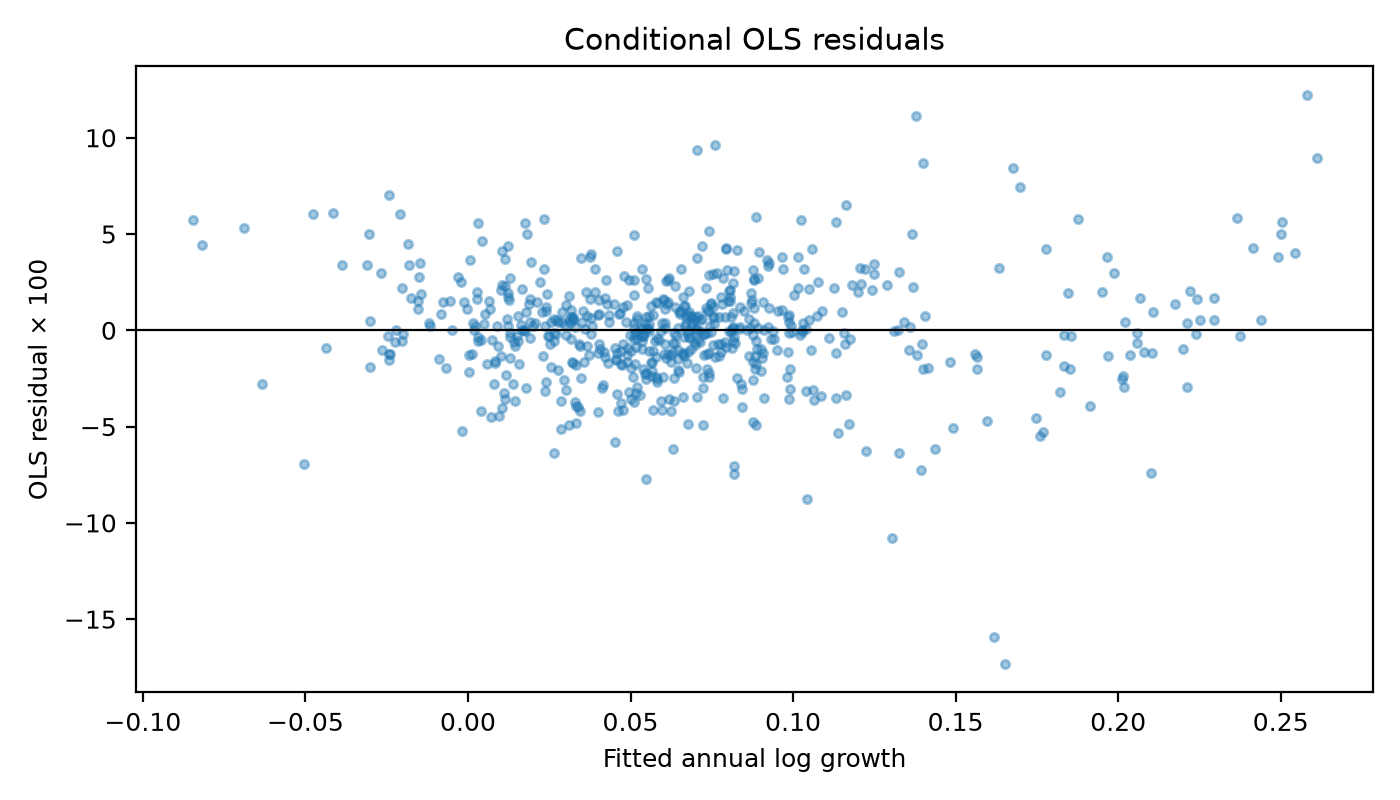
\includegraphics[width=0.80\linewidth]{ols_residuals.png}
\caption{Conditional OLS fitted growth and residuals. The spread and remaining geography of residuals motivate spatial diagnostics.}
\label{fig:residuals}
\end{figure}

\section{Robustness and sensitivity}
\begin{table}[htbp]
\centering\small
\caption{Sensitivity of the conditional initial-light coefficient}
\begin{tabular}{lrrr}
\toprule
Specification & Districts & OLS coefficient (HC3 SE) & SAR $\rho$\\
\midrule
Main VIIRS, 2013--2021 & 640 & $-0.04569\ (0.00344)$ & 0.1966\\
VIIRS median-masked, 2013--2021 & 640 & $-0.04579\ (0.00351)$ & 0.2142\\
VIIRS average, 2014--2019 & 640 & $-0.05358\ (0.00440)$ & 0.2517\\
VIIRS average, eight-nearest-neighbor $W$ & 640 & $-0.04569\ (0.00344)$ & 0.1406\\
VIIRS average, two-year-smoothed endpoints & 640 & $-0.04453\ (0.00356)$ & 0.2380\\
VIIRS average, Queen non-islands only & 628 & $-0.04600\ (0.00346)$ & 0.1842\\
Calibrated DMSP, 2000--2013 & 640 & $-0.02595\ (0.00259)$ & 0.4504\\
VIIRS, omit top/bottom 1\% growth & 626 & $-0.04213\ (0.00324)$ & --\\
\bottomrule
\end{tabular}
\label{tab:robust}
\end{table}

The sign of the initial-light association persists with the alternative VIIRS mask, a pre-2020 period, graph changes, and trimming extreme growth observations. The DMSP result is a separate historical analogue; its level, growth rate, and spatial parameter should not be compared numerically with VIIRS because sensor resolution, dynamic range, and calibration differ. The eight-neighbor graph connects districts separated by sea or geometry gaps, so it tests sensitivity to geographic definition rather than identifying a superior physical diffusion channel.

\section{Limitations and conclusions}
The analysis is descriptive and conditional, not causal. Night-light intensity is affected by electrification, lighting technology, saturation, blooming, cloud and masking rules, and location-specific economic composition. A fixed 2011 population denominator cannot represent population growth or migration during 2013--2021. State indicators absorb state-wide differences but not district-specific omitted variables or correlated shocks. Spatial-lag outcomes are simultaneous, and Gaussian ML inference can be sensitive to error misspecification. Multiple spatial-weight choices are plausible. Local clusters depend on the same measurement and weight definitions.

Within these limits, the evidence is clear on three narrower points: normalized night lights rose in most districts; lower initially lit districts had higher subsequent light growth; and growth was strongly spatially patterned. Models that allow spatial error or Durbin dependence account for much of the residual pattern. The extra spatial grouping analysis reveals broad regional types but with weak feature separation. A stronger economic-convergence claim would require validated district output or consumption outcomes, annual population estimates, and a design that isolates exogenous sources of neighboring growth.

\section*{Reproducibility and rights}
All data joins, figures, permutation tests, regressions, likelihood comparisons, impact calculations, and cluster assignments are generated from the included Python scripts and derived panels. The data and district geometry originate from SHRUG v2.2 and retain its CC BY-NC-SA 4.0 noncommercial, attribution, and share-alike terms \cite{shruglicense}. The source files, variable choices, checks, and software versions are listed in \path{DATA_SOURCES.md} and \path{requirements.txt} in the repository. This report was prepared without using the ambiguous historical SHRID-to-district crosswalk for the main 2013--2021 denominator.

\begin{thebibliography}{9}
\bibitem{asher2021} Asher, S., Lunt, T., Matsuura, R., and Novosad, P. (2021). Development Research at High Geographic Resolution: An Analysis of Night-Lights, Firms, and Poverty in India Using the SHRUG Open Data Platform. \emph{World Bank Economic Review}, 35(4), 845--871. \url{https://doi.org/10.1093/wber/lhab003}.
\bibitem{henderson2012} Henderson, J. V., Storeygard, A., and Weil, D. N. (2012). Measuring Economic Growth from Outer Space. \emph{American Economic Review}, 102(2), 994--1028. \url{https://doi.org/10.1257/aer.102.2.994}.
\bibitem{shrugviirs} Development Data Lab. SHRUG v2.2: VIIRS Annual Night Lights district metadata. \url{https://docs.devdatalab.org/SHRUG-Metadata/Night-time\%20lights/Tables/viirs-annual-metadata/}.
\bibitem{shrugdmsp} Development Data Lab. SHRUG v2.2: DMSP Night Lights district metadata. \url{https://docs.devdatalab.org/SHRUG-Metadata/Night-time\%20lights/Tables/dmsp-metadata/}.
\bibitem{shruglicense} Development Data Lab. SHRUG v2.2 license and terms. \url{https://docs.devdatalab.org/Getting-Started/license/}.
\bibitem{pysalimpact} PySAL \texttt{spreg}. Maximum-likelihood spatial lag estimation and spatial impacts. \url{https://pysal.org/spreg/notebooks/13_ML_estimation_spatial_lag.html}.
\end{thebibliography}
\end{document}
